% !Mode:: "TeX:UTF-8"
%!TEX program  = xelatex

%\documentclass[bwprint,fontset=windows]{gmcmthesis}
\documentclass[bwprint]{gmcmthesis}

\hypersetup{hidelinks}
\usepackage[framemethod=TikZ]{mdframed}

%\usepackage{fontspec}  % for Consolas & Courier New
%\lstset{basicstyle=\small\fontspec{Consolas}}
%\lstset{basicstyle=\small\fontspec{Courier New}}
%\setmonofont{Consolas}
%\setcounter{tocdepth}{3}   % 调整目录深度

\usepackage{subfig}
\usepackage{siunitx}

\usepackage{colortbl}
\definecolor{color1}{rgb}{0.78,0.88,0.99}
\definecolor{color2}{rgb}{0.36,0.62,0.84}
%\definecolor{color3}{rgb}{0.8235,0.8706,0.9373}
\definecolor{color3}{rgb}{0.88,0.92,0.96}
\definecolor{color4}{rgb}{0.96,0.97,0.98}%{0.9176,0.9373,0.9686}

% 算法
\usepackage[noend]{algpseudocode}
\usepackage{algorithmicx,algorithm}
\floatname{algorithm}{算法}
\renewcommand{\algorithmicrequire}{\textbf{输入:}}
\renewcommand{\algorithmicensure}{\textbf{输出:}}

%\numberwithin{equation}{section}
%\numberwithin{figure}{section}
%\numberwithin{table}{section}


\newcommand{\red}[1]{\textcolor{red}{#1}}
\newcommand{\blue}[1]{\textcolor{blue}{#1}}


%===================== 建模论文题目 ======================

\title{全国研究生数学建模竞赛论文标题}
\baominghao{\hspace{6em} 00000000001} %参赛队号
\schoolname{\hspace{5.8em} 学校名称填写} %学校名称
\membera{\hspace{6em} 成员A} %队员A
\memberb{\hspace{6em} 成员B} %队员B
\memberc{\hspace{6em} 成员C} %队员C

%=======================================================


\begin{document}

%生成标题
\maketitle

%填写摘要
\begin{abstract}
本模板是为全国研究生数学建模竞赛编写的 \LaTeX{} 模板, 旨在让大家专注于
论文的内容写作, 而不用花费过多精力在格式的定制和调整上. 本手册是相应的参考, 其
中提供了一些环境和命令可以让模板的使用更为方便. 同时需要注意, 使用者需要有一
定的 \LaTeX{} 的使用经验, 至少要会使用 ctex 宏包的一些功能, 比如调节字距或修改字体
大小等等.

\begin{mdframed}[%
roundcorner=5pt,linecolor=gray!50,outerlinewidth=0.5pt,
middlelinewidth=0.3pt,backgroundcolor=gray!2,
innertopmargin=\topskip, frametitle={2025年格式变化说明},
frametitlefont= \bfseries,frametitlerule=true,frametitlealignment =\raggedright\noindent,
frametitlerulewidth=.5pt, frametitlebackgroundcolor=gray!2,]
今年的格式变化如下:
\begin{enumerate}
\item 论文前两页 Logo 和 Title 替换;
\end{enumerate}
\end{mdframed}

这是研究生报名官方网站,点击\href{https://cpipc.acge.org.cn/}{\fbox{这里}}进入。


\keywords{食堂打饭\quad  明德中学\quad   非线性优化模型\quad  多属性决策}

\end{abstract}

\pagestyle{plain}

%目录 不推荐加
\maketoc

\clearpage

\section{问题重述}

\subsection{引言}   % 问题的背景

午休铃刚响,明德中学的食堂就炸开了锅。初三(2)班的林晓宇抱着饭盒冲进人群,看着每条队伍都像蜿蜒的长蛇,不禁叹气:“每天都要花 20 分钟排队,作业都要写不完了!” 同桌陈默推了推眼镜:“说不定,我们能用数学建模解决这个问题?”


\subsection{问题的提出}

%\subsubsection{问题的提出内容一}

\noindent 明德中学食堂每日午休时段(12:00-12:30)、晚餐时段(18:00-18:30)人流高度集中,6 个打饭窗口前均出现长队。经初步统计,学生平均排队等待时间达 20 分钟,部分学生因排队错过午休,或因担心迟到放弃堂食。

\textbf{问题一:} 学生选择队伍的盲目性(仅依据队伍长度,忽略窗口打饭速度差异)。在明德中学食堂高峰时段,学生选择打饭队伍时,普遍存在“以长度论快慢”的盲目决策现象。比如午休12:05左右,食堂6个窗口中,$W_5$(汤类窗口)前排队人数为8人,$W_1$(主食窗口)前排队人数为10人,多数学生会优先选择$W_5$队伍——仅因直观上“少2人”,却忽略了两个窗口的打饭速度差异:$W_1$平均30秒就能为1名学生打饭(主食只需快速舀取米饭/馒头),而$W_5$因需逐个盛汤、加配料,平均1分30秒才能服务1人。

\textbf{问题二:} 窗口功能分配不合理(慢窗口集中导致局部拥堵)
食堂现有窗口布局为“横向连续排列”,且功能分配存在明显的“快慢扎堆”问题:6个窗口从左到右依次为$W_1$(主食,快)、$W_2$(菜品,中慢)、$W_3$(菜品,中慢)、$W_4$(主食,快)、$W_5$(汤类,慢)、$W_6$(特色菜,慢)。其中,$W_2,W_3$(中慢窗口)集中在中间区域,$W_5,W_6$(慢窗口)集中在右侧区域,形成了两个明显的“拥堵带”。

\textbf{问题三:} 缺乏对人流规律与等待时间的量化分析,无法针对性优化。
食堂仅知道“午休、晚餐人多”,却不清楚具体高峰时段的人流峰值(如午休12:08-12:15为人流最高峰,到达率达0.4人/秒,远超其他时段的0.2人/秒)、不同年级学生的就餐偏好(初三学生因作业多,多在12:00-12:10集中就餐,初一学生则分散在12:10-12:25),无法根据人流波动调整窗口开放数量(如高峰时开6个窗口,平峰时开3个)。


\clearpage
\section{模型的假设}
为简化问题、聚焦核心矛盾,建立以下假设:
\begin{enumerate}
\item 人流分布假设:学生到达食堂的时间服从泊松分布,即任意时间段内到达的学生数量相互独立,无集中 “批量到达”(如整班集体前往);
\item 窗口效率假设:同一窗口的打饭速度稳定(如主食窗口平均 30 秒 / 人,菜品窗口平均 1 分钟 / 人),无突发故障(如餐具短缺导致速度骤降);
\item 学生选择假设:学生仅依据 “当前队伍长度” 选择窗口,不了解历史等待数据,且选择后不更换队伍;
\item 时间范围假设:仅研究人流高峰时段(午休 12:00-12:30、晚餐 18:00-18:30),非高峰时段(如 12:30 后)人流稀疏,无需优化。
\end{enumerate}




\section{符号说明}

\begin{table}[htp!]
\centering
\renewcommand\arraystretch{1.2} %定义表格高度
\newcolumntype{L}{>{\quad}X}
\newcolumntype{P}[1]{>{\centering\arraybackslash}p{#1}}
\newcolumntype{C}{>{\centering \arraybackslash}X}
\newcolumntype{R}{>{\raggedright \arraybackslash}X}
\begin{tabularx}{0.9\textwidth}{|P{1cm}|L|}
  \hline %\toprule
  符号    &   \quad 意义 \\
  \hline %\midrule
  %\rowcolor[gray]{0.90}
  $ a $  &  符号1的意义    \\
  \hline
  $ b $  &  符号2的意义    \\
  \hline
  $ c $  &  符号3的意义符号3的意义    \\
  \hline
  $ d $  &  符号4的意义    \\
  \hline
  $ e $  &  符号5的意义     \\
  \hline
  $ f $  &  符号6的意义符号6的意义    \\
  \hline
  $ g $  &  符号7的意义     \\
  \hline
  $ h $  &  符号8的意义     \\
  \hline
  $ i $  &  符号9的意义符号9的意义     \\
  \hline

  $ k $  &  符号10的意义     \\
  \hline
  $ l $  &  符号11的意义    \\
  \hline
  $ m $  &  符号12的意义    \\
  \hline
  $ n $  &  符号13的意义    \\
  \hline
  $ p $  &  符号14的意义    \\
  \hline
  $ q $  &  符号15的意义    \\
  \hline %\bottomrule
\end{tabularx}
\end{table}


%\begin{tabularx}{\textwidth-18pt}{XXX}
%\hline
%Input & Output& Action return \\
%\hline
%DNF &  simulation & jsp\\
%\hline
%\end{tabularx}


\section{模型的建立}

\subsection{问题一分析}
题目要求建立模型描述折叠桌的动态变化图,由于在折叠时用力大小的不同,我们不能描述在某一时刻折叠桌的具体形态,但我们可以用每根木条的角度变化来描述折叠桌的动态变化。首先,我们知道折叠桌前后左右对称,我们可以运用几何知识求出四分之一木条的角度变化。最后,根据初始时刻和最终形态两种状态求出桌腿木条开槽的长度


\subsection{算法示例}

数学建模求解算法示例:
\begin{center}
\begin{minipage}{0.8\textwidth}
\begin{algorithm}[H]%[!htp]
\caption{算法的名字} %算法的名字
{\bf 输入:} %算法的输入, \hspace*{0.02in}用来控制位置,同时利用 \\ 进行换行
input parameters A, B, C\\
{\bf 输出:} %算法的结果输出
output result
\begin{algorithmic}[1]
\State some description 算法介绍 % \State 后写一般语句
\For{condition} % For 语句,需要和EndFor对应
  \State ...
  \If{condition} % If 语句,需要和EndIf对应
    \State ...
  \Else
    \State ...
  \EndIf
\EndFor
\While{condition} % While语句,需要和EndWhile对应
  \State ...
\EndWhile
\State \Return result
\end{algorithmic}
\end{algorithm}
\end{minipage}
\end{center}
\vspace{2ex}

多属性决策算法通过对每个决策选项(即各打饭窗口)的多个属性(队伍长度、服务效率)进行加权计算,得到每个选项的综合得分,得分最高的选项即为最优选择。在食堂排队场景中,需先定义属性权重(根据学生对“等待时间”的敏感度设定),再通过标准化处理消除属性单位差异,最终计算综合得分。


\textbf{步骤1:计算各窗口预估等待时间} \\
  预估等待时间$T_i$反映该窗口的实际等待成本,计算公式为:
  \[
  T_i = \frac{L_i}{v_i}
  \]
  示例:$T_1 = \frac{10}{2} = 5$分钟(主食窗口),$T_5 = \frac{8}{0.67} \approx 12$分钟(汤类窗口)。

\textbf{步骤2:属性标准化处理} \\
  因“队伍长度”“服务效率”单位不同,需标准化为$[0,1]$区间的得分(得分越高,属性越优):
  1. 队伍长度标准化得分(长度越短,得分越高):
     \[
     S_{L_i} = \frac{\max(L_i) - L_i}{\max(L_i) - \min(L_i)}
     \]
     示例:若当前窗口最大长度$\max(L_i)=10$,最小$\min(L_i)=8$,则$S_{L_1} = \frac{10-10}{10-8} = 0$,$S_{L_5} = \frac{10-8}{10-8} = 1$。
  2. 服务效率标准化得分(效率越高,得分越高):
     \[
     S_{v_i} = \frac{v_i}{\max(v_i)}
     \]
     示例:$\max(v_i)=2$(主食窗口),则$S_{v_1} = \frac{2}{2} = 1$,$S_{v_5} = \frac{0.67}{2} \approx 0.33$。

\textbf{步骤3:计算窗口综合得分} \\
  综合得分$S_i$为各属性标准化得分的加权和,得分越高,窗口越优:
  \[
  S_i = w_1 \times S_{L_i} + w_2 \times S_{v_i}
  \]
  示例:$S_1 = 0.4 \times 0 + 0.6 \times 1 = 0.6$,$S_5 = 0.4 \times 1 + 0.6 \times 0.33 \approx 0.598$。


\section{表格和图形}

\subsection{表格}

使用 tabular 环境, 如下表格: 表~\ref{tab:foo}. 通过 \verb|autoref| 引用表格: \autoref{tab:foo}.

这里可使用命令 \verb|\tabcolsep| 和 \verb|\arraystretch| 分别控制列间距和行间距.

\begin{table}[htp!]
\centering
\setlength{\tabcolsep}{12pt}  % 6pt standard
\renewcommand{\arraystretch}{1.2}
\caption{学术活动安排样例}
\label{tab:foo}
\begin{tabular}{|c|c|c|c|}
\hline
\textbf{日期}  & \textbf{地点} & \textbf{活动名称} & \textbf{备注} \\ \hline
2024年8月1日      & 上海       & 学术研讨会      & 主题:人工智能 \\ \hline
2024年8月15日    & 北京       & 学术交流会      & 重点:数学建模 \\ \hline
2024年9月1日      & 深圳       & 研究研讨会      & 主题:数据科学 \\ \hline
2024年10月15日  & 广州       & 创新论坛         & 重点:科技创新 \\ \hline
\end{tabular}
\end{table}


\clearpage

三线表
\begin{table}[htp!]
\newcolumntype{L}{X}
\newcolumntype{C}{>{\centering \arraybackslash}X}
\newcolumntype{R}{>{\raggedright \arraybackslash}X}
\centering
\caption{某校学生升高体重样本}
\label{tab:heightweight}
\begin{tabularx}{0.9\textwidth}{CCCC}
\toprule
序号 & 年龄 & 身高 & 体重 \\
\midrule
001 & 15 & 156 & 42 \\
002 & 16 & 158 & 45 \\
003 & 14 & 162 & 48 \\
004 & 15 & 163 & 50 \\
\cmidrule{2-4}
平均 & 15 & 159.75 & 46.25 \\
\bottomrule
\end{tabularx}
\end{table}

% 某行业产量与生产费用的数据
% \begin{table}[htp!]
% \centering
% \caption{某行业产量与生产费用的数据}%\label{}
% \newcolumntype{Y}{>{\centering\arraybackslash}X}
% \newcolumntype{Z}{!{\vline}@{\color{white}\vrule width \doublerulesep}!{\vrule}}%自定义列格式(双线)
% \begin{tabularx}{0.94\textwidth}{c|c|YZc|c|Y}
% \Xhline{0.9pt}
% 企业编号&  产量(台)&生产费用(万元)&企业编号&产量(台)&生产费用(万元)\\\Xcline{1-3}{0.6pt}\Xcline{4-6}{0.6pt}
% 1 & 40 & 130 & 7&  84&  165\\
% 2 & 42 & 150 & 8&  100&  170\\
% 3 & 50 & 155 & 9&  116&  167\\
% 4 & 55 & 140 & 10&  125&  180\\
% 5 & 65 & 150 & 11&  130&  175\\
% 6 & 78 & 154 & 12&  140&  185\\\Xhline{0.72pt}
% \end{tabularx}
% \end{table}

研究生数学建模2019年F题结果示例
\begin{table}[htp!]
\centering
\caption{问题1结果1 (左) 与 问题2结果 (右)}
\begin{minipage}[h]{0.48\linewidth}
\renewcommand\arraystretch{1.2} %定义表格高度
\newcolumntype{Y}{>{\centering\arraybackslash}X}
\begin{tabularx}{0.9\textwidth}{|Y|Y|Y|}
  \hline
  数据集1  &  数据集1 & 数据集2  \\
 \hline
  A问题1   & A问题1 &  A问题1     \\
  \hline
  503   &  503     & 163     \\
  294   &  200     & 114      \\
  91    &  80      & 8     \\
  607   &  237     & 309      \\
  540   &  170     & 305    \\
  250   &  278     & 123    \\
  340   &  369     & 45      \\
  277   &  214     & 160    \\
  B     &  397     & 92    \\
        &  B       & 93    \\
        &          & 61        \\
        &          & 292       \\
        &          & B         \\
104861  & 103518   & 109342 \\
\hline
\end{tabularx}
\end{minipage}
\begin{minipage}[h]{0.48\linewidth}
\renewcommand\arraystretch{1.2} %定义表格高度
\newcolumntype{Y}{>{\centering\arraybackslash}X}
\begin{tabularx}{0.9\textwidth}{|Y|Y|Y|}
  \hline
  数据集1  &  数据集1 & 数据集2  \\
  \hline
  A问题2  &  A问题2  & A问题2    \\
  \hline
   503    & 503     & 163  \\
  294    & 200     & 114   \\
   91     & 80     & 8   \\
   607    & 237     & 309   \\
   540    & 170    & 305  \\
   250    & 278    & 123  \\
   340    & 369     & 45   \\
   277    & 214    & 160  \\
  B      & 397   & 92 \\
        &  B     &  93      \\
         &         &  61      \\
        &         &   292     \\
        &         &   B     \\
 104917  &  103563  &109427 \\
\hline
\end{tabularx}
\end{minipage}
\end{table}

\clearpage
\begin{table}[htp!]
%\small
\centering
\renewcommand\arraystretch{1.2} %定义表格高度
\newcolumntype{Y}{>{\centering\arraybackslash}X}
\caption{问题3结果}
\begin{tabularx}{0.9\textwidth}{|Y|Y|Y|Y|Y|Y|}
  \hline %定义表格宽度
  数据集1  &  数据集1  &  \multicolumn{2}{c|}{数据集2 (无问题点)}  & \multicolumn{2}{c|}{数据集2 (有问题点)} \\
  \hline
  A问题3   & A问题3   &  \multicolumn{2}{c|}{A问题3}    &  \multicolumn{2}{c|}{A问题3}      \\
  \hline
  503      & 503     & 169      & 73      & 169     & 73   \\
  \hline
  69       & 69      & 322      & 249     & 322     & 249   \\
  \hline
  506      & 506      & 270     & 274     & 270     & 274   \\
  \hline
  371      & 371      & 89      & 12      & 89      & 12   \\
  \hline
  183      & 183      & 236     & 216     & 236     & 216  \\
  \hline
  194      & 194      & 132     & 16      & 132     & 16   \\
  \hline
  450      & 450      & 53      & 282     & 53      & 282   \\
  \hline
  286      & 113      & 112     & 84      & 112     & 141  \\
  \hline
  485      & 485      &  268    & 287     & 268     & 291 \\
  \hline
 \red{B (9D)}~~     & 248      & 250     & 99      & 250     &161 \\
 \hline
   & \red{B (10D)}   & 243     & \red{B (21D)}   & 243    & \red{B (21D)} \\
   \hline
    &          &         &         &         &       \\
    \hline
  104861m  & 103518m  &         & 168924m  &         &161650m \\
\hline
\end{tabularx}
\end{table}


\subsection{图形}

图形并列
\begin{figure}[htp!]
\begin{minipage}[t]{0.48\linewidth}
\centering
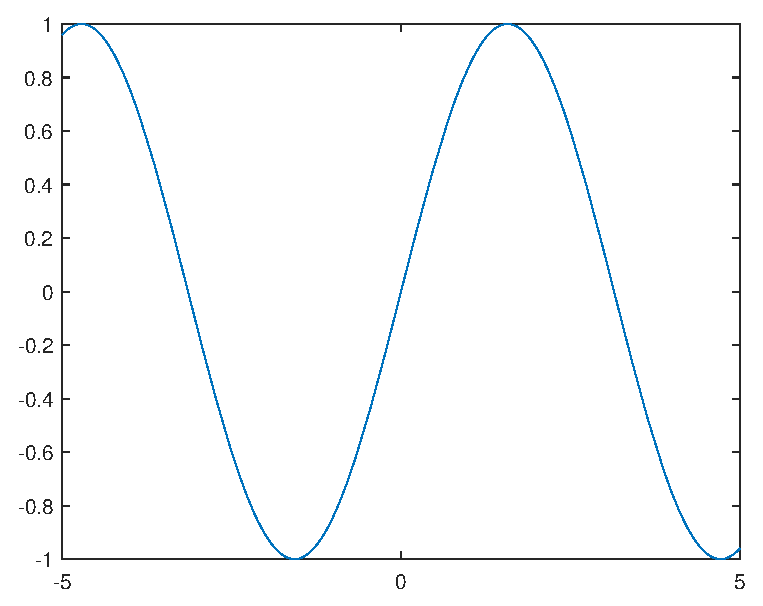
\includegraphics[width=0.9\textwidth]{image1}
\caption{fig1}
\label{fig:side:a}
\end{minipage}%
\begin{minipage}[t]{0.48\linewidth}
\centering
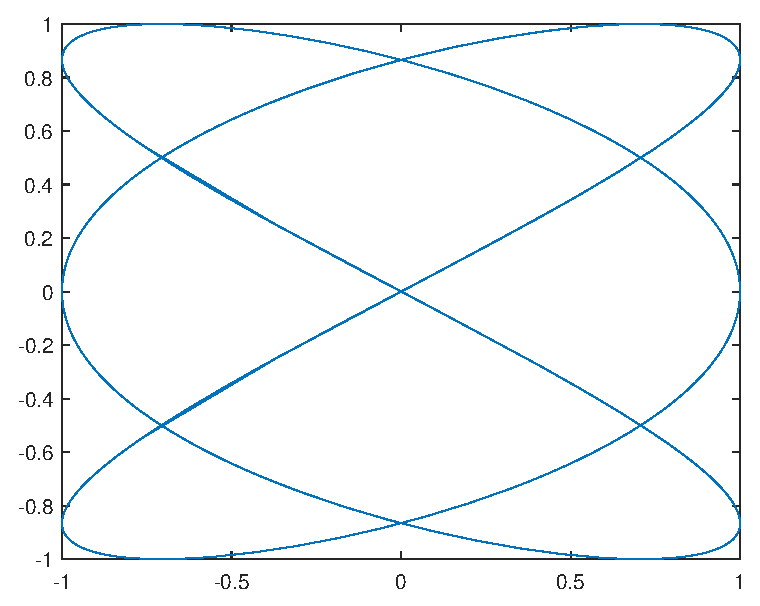
\includegraphics[width=0.9\textwidth]{image2}  % 2.2in
\caption{fig2}
\label{fig:side:b}
\end{minipage}
\end{figure}

这是一个算法流程图
\begin{figure}[htp!]
\centering
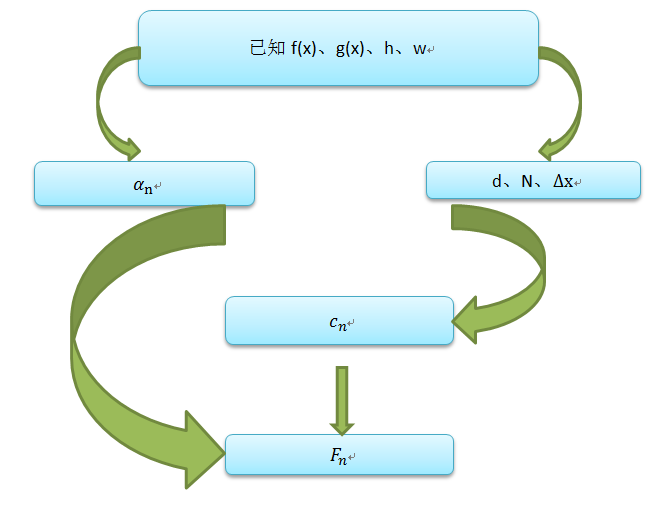
\includegraphics[width=.55\textwidth]{fig.png}
\caption{算法流程图}
\end{figure}

多图并排
\begin{figure}[!htp]
	\centering
	\subfloat[Arabic numerals]{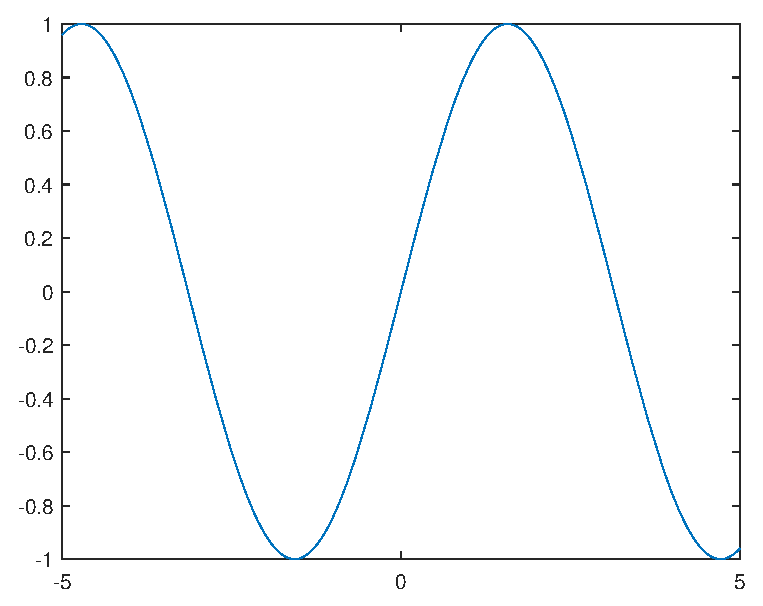
\includegraphics[width=0.4\textwidth]{image1}}\qquad
	\subfloat[Arabic numerals]{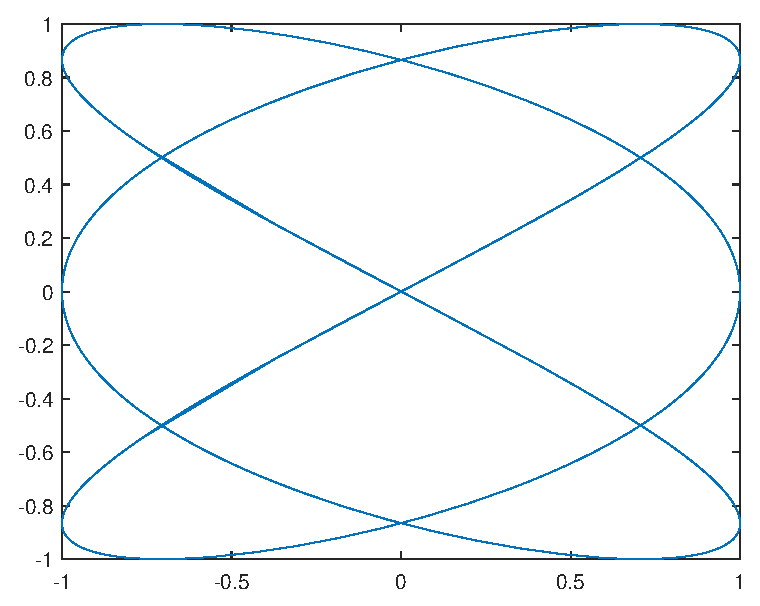
\includegraphics[width=0.4\textwidth]{image2}} \\
	\subfloat[Arabic numerals]{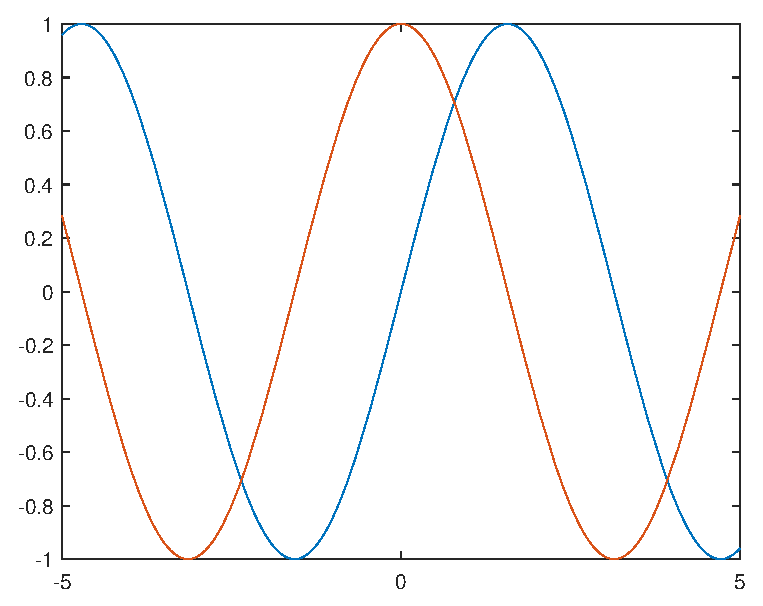
\includegraphics[width=0.4\textwidth]{image3}}\qquad
	\subfloat[Arabic numerals]{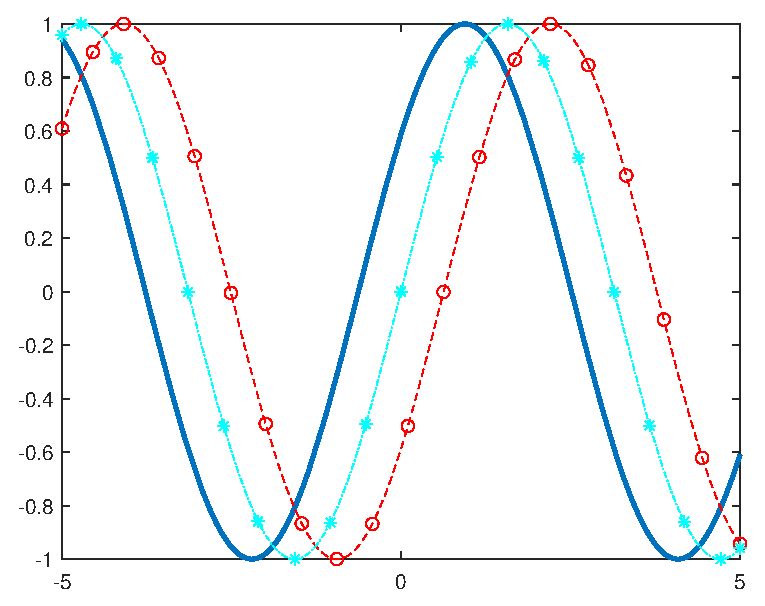
\includegraphics[width=0.4\textwidth]{image4}}
	\caption{多图示例}
\end{figure}


\clearpage


\section{模型评价}

这里是模型评价



%参考文献   手工录入
%\begin{thebibliography}{9}%宽度9
% \bibitem{bib:one} ....
% \bibitem{bib:two} ....
%\end{thebibliography}

%采用bibtex方案
\cite{mittelbach_latex_2004,wright_latex3_2009,beeton_unicode_2008,vieth_experiences_2009}

\bibliographystyle{gmcm}
\bibliography{reference}


\clearpage
%附录
\begin{appendices}
%\setcounter{page}{1} %如果需要可以自行重置页码。
\section{MATLAB 源程序}
\renewcommand{\thesubsection}{A\thinskip.\thinskip\arabic{subsection}}
\subsection{第1问程序}
\vspace{-2ex}

\begin{Matlab}{code.m}
clear all
kk=2;
[mdd,ndd]=size(dd);
while ~isempty(V)
    [tmpd,j]=min(W(i,V));
    tmpj=V(j);
    for k=2:ndd
        [tmp1,jj]=min(dd(1,k)+W(dd(2,k),V));
        tmp2=V(jj);
        tt(k-1,:)=[tmp1,tmp2,jj];
    end
    tmp=[tmpd,tmpj,j;tt];
    [tmp3,tmp4]=min(tmp(:,1));
    if tmp3==tmpd,
        ss(1:2,kk)=[i;tmp(tmp4,2)];
    else
        tmp5=find(ss(:,tmp4)~=0);
        tmp6=length(tmp5);
        if dd(2,tmp4)==ss(tmp6,tmp4)
            ss(1:tmp6+1,kk)=[ss(tmp5,tmp4);tmp(tmp4,2)];
        else, ss(1:3,kk)=[i;dd(2,tmp4);tmp(tmp4,2)];
        end
    end
    dd=[dd,[tmp3;tmp(tmp4,2)]];
    V(tmp(tmp4,3))=[];
    [mdd,ndd]=size(dd);kk=kk+1;
end;
S=ss; D=dd(1,:);
\end{Matlab}
\vspace{2ex}

\clearpage
\section{Python 源程序}
\renewcommand{\thesubsection}{B\thinskip.\thinskip\arabic{subsection}}
\subsection{第2问程序}
\vspace{-2ex}
\begin{Python}{mip1.py}
# This example formulates and solves the following simple MIP model:
#  maximize
#        x +   y + 2 z
#  subject to
#        x + 2 y + 3 z <= 4
#        x +   y       >= 1
#        x, y, z binary

# import gurobipy as gp
from gurobipy import * #GRB
try:
    # Create a new model
    m = Model("mip1")
    # Create variables
    x = m.addVar(vtype=GRB.BINARY, name="x")
    y = m.addVar(vtype=GRB.BINARY, name="y")
    z = m.addVar(vtype=GRB.BINARY, name="z")
    # Set objective
    m.setObjective(x + y + 2 * z, GRB.MAXIMIZE)
    # Add constraint: x + 2 y + 3 z <= 4
    m.addConstr(x + 2 * y + 3 * z <= 4, "c0")
    # Add constraint: x + y >= 1
    m.addConstr(x + y >= 1, "c1")
    # Optimize model
    m.optimize()
    for v in m.getVars():
        print('%s %g' % (v.varName, v.x))
    print('Obj: %g' % m.objVal)

except GurobiError as e:
    print('Error code ' + str(e.errno) + ': ' + str(e))

except AttributeError:
    print('Encountered an attribute error')
\end{Python}

\end{appendices}



\end{document}
